\begin{figure}[t]
\centering
\subfloat[Exact optimal cost v.s. heuristic approximation using clustering]{
    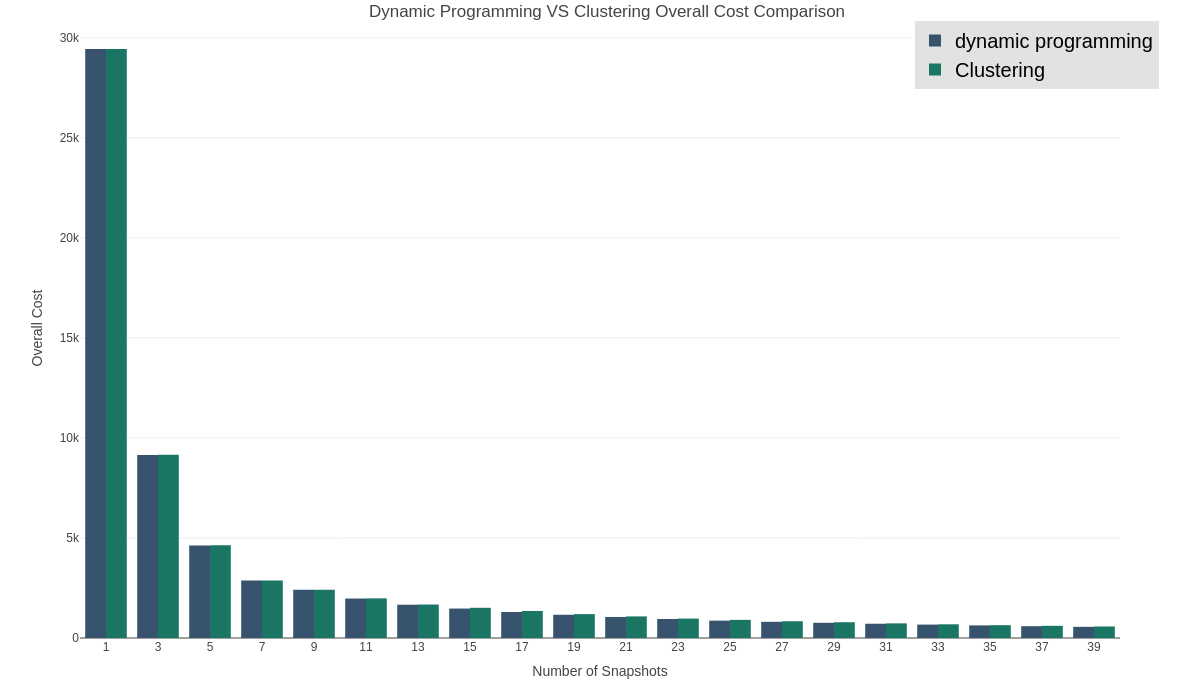
\includegraphics[width=0.45\linewidth]{figs/dynamic_vs_clustering.jpg}
    \label{fig:place-1}
}
\hfill
\subfloat[Approximation quality of 300 iterations vs 5 iterations] {
    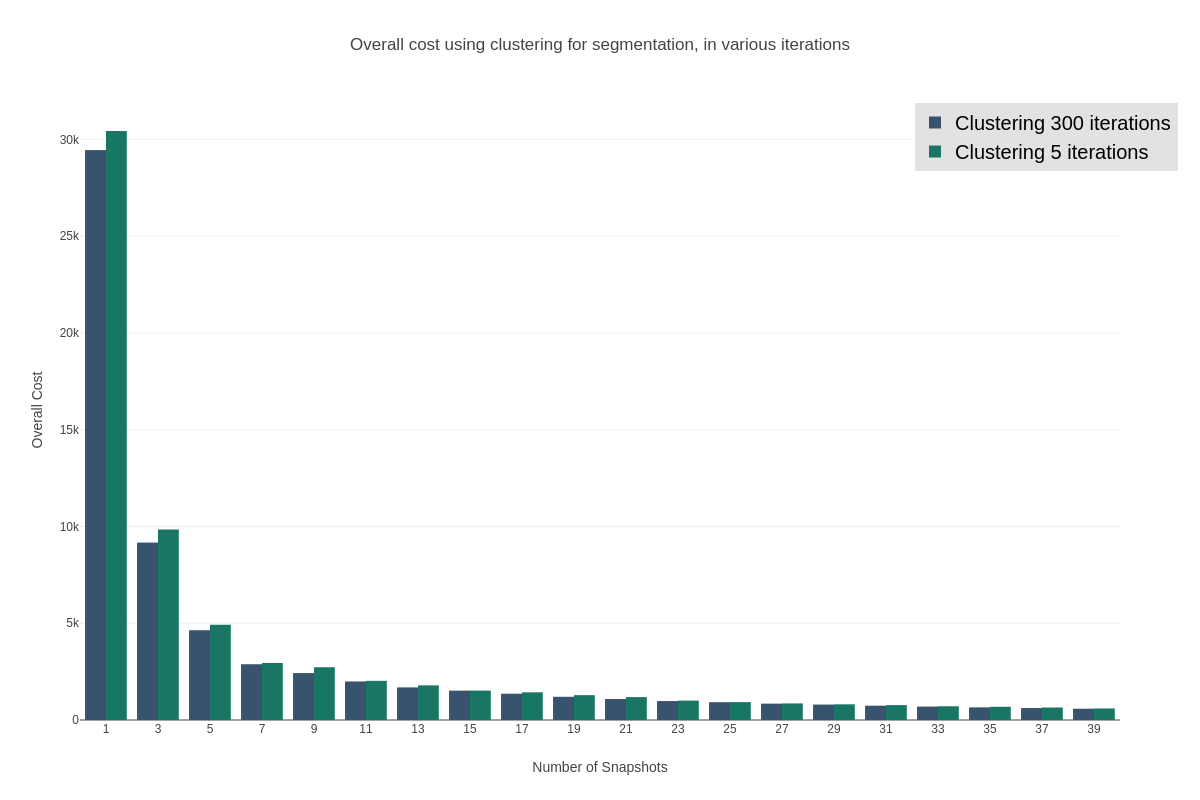
\includegraphics[width=0.45\linewidth]{figs/compare_clustering_iterations.png}
    \label{fig:place-2}
}
    \caption{Quality of the approximate snapshot placements using clustering}
    \label{fig:place}
\end{figure}

\section{Evaluation and experiments}

We have conducted a number of experiments to evaluate the effectiveness of the
proposed algorithms.

A synthetic query workload is generated against a database with over 1
million tuples.  Figure~\ref{fig:query-answer} shows the benefit of having
optimally placed snapshots.  Figure~\ref{fig:query-answer-1} shows the effect of
having just a single snapshot.  One can see that the cost is minimal when the
materialized snapshot is at the median of the query workload.
Figure~\ref{fig:query-answer-2} shows the benefit of having more snapshots
optimally materialized.  We see that with 40 materialized snapshots, the cost is
reduced to less than
2\% when compared to just one materialized snapshot.
Figure~\ref{fig:query-answer-3} shows the
relative performance of different snapshot placement strategies.  We see that
random placements and fixed interval placements are significant worse than the
optimal placement strategy, with the cost being over 15 times worse.

We have compared the runtime performance of the optimal snapshot placement using
dynamic programming and clustering based heuristics.  Figure~\ref{fig:runtime-1}
compares the runtime performance of dynamic programming and clustering with 300
iterations.  One can see that the clustering heuristics scales extremely well
with increasing query workload size.  To further speedup the snapshot placement
computation, we can reduce the number of iterations further as shown in
Figure~\ref{fig:runtime-2}.

The heuristic approach is highly effective in obtaining near optimal snapshot
placements. Figure~\ref{fig:place-1} compares the costs of optimal placements and
approximate placements using 300 iterations.  The increase in the cost is less
than 2\%.  Even with just 5 iterations, as shown in Figure~\ref{fig:place-2}, the
resulting approximation is very close to the exact optimal placement.
